% ── Chapter 4: Results and Discussion ────────────────────────
\chapter{Results and Discussion}

This chapter presents the experimental results for each major component of the system:
object detection and ZOI measurement, dataset size effects on training, OCR performance,
pixel-to-millimeter calibration, end-to-end processing speed, user evaluation,
and web application completeness.
All quantitative results are reported on the held-out test partition unless stated otherwise.

% ─────────────────────────────────────────────────────────────
\section{Object Detection Performance}
\label{sec:detection_performance}
% ─────────────────────────────────────────────────────────────

Table~\ref{tab:model_comparison} summarizes the ZOI detection results across the two deep learning
models, showing the measured diameter versus the expert ground-truth (GT) diameter
for four antibiotics: Penicillin (P), Oxacillin (OX), Chloramphenicol (C), and Kanamycin (CN).
Two measurement strategies are reported for each model:
an \emph{area-based} estimate derived from the bounding-box area
and a \emph{diameter-based} estimate derived directly from the predicted bounding-box width.
The error columns show the signed difference (model minus expert GT); positive values indicate
overestimation and negative values indicate underestimation.

\noindent\textbf{Note:} YOLOv11n detailed MAE was not reported in the Term~1 evaluation
and is shown as ``---'' throughout. Quantitative MAE for YOLOv11n represents ongoing
evaluation in the Term~2 phase of the project.

\begin{table}[H]
  \centering
  \caption{ZOI Measurement Results --- Per-Antibiotic Comparison (all values in mm).
           Expert GT is the single consensus diameter from the clinical expert.
           ``Diam.'' columns use the bounding-box width directly;
           ``Area'' columns derive the effective diameter from the bounding-box area.
           Error = Model $-$ Expert GT (positive = overestimation).
           YOLOv11n demonstrates superior accuracy with a mean absolute error (MAE) of approximately 2.5--2.7 mm.}
  \label{tab:model_comparison}
  \renewcommand{\arraystretch}{1.15}
  \begin{tabular}{lccccccccc}
    \toprule
    \multirow{2}{*}{\textbf{Antibiotic}} &
    \multirow{2}{*}{\textbf{Expert GT}} &
    \multicolumn{2}{c}{\textbf{FRCNN}} &
    \multicolumn{2}{c}{\textbf{YOLOv11n}} &
    \multicolumn{2}{c}{\textbf{FRCNN Error}} &
    \multicolumn{2}{c}{\textbf{YOLO Error}} \\
    \cmidrule(lr){3-4}\cmidrule(lr){5-6}\cmidrule(lr){7-8}\cmidrule(lr){9-10}
    & & Diam. & Area & Diam. & Area & Diam. & Area & Diam. & Area \\
    \midrule
    P  (Penicillin)       & 38 & 30.52 & 30.06 & 37.84 & 33.54 & $+$7.48 & $+$7.94 & $+$0.16 & $+$4.46 \\
    OX (Oxacillin)        & 30 & 25.69 & 25.30 & 33.62 & 29.80 & $+$4.31 & $+$4.69 & $-$3.62 & $+$0.20 \\
    C  (Chloramphenicol)  & 20 & 14.68 & 14.46 & 17.00 & 15.07 & $+$5.32 & $+$5.54 & $+$3.00 & $+$4.93 \\
    CN (Kanamycin)        & 17 & 18.50 & 18.21 & 20.93 & 18.55 & $-$1.50 & $-$1.21 & $-$3.93 & $-$1.55 \\
    \midrule
    \textbf{Bias}         & --- & \multicolumn{2}{c}{} & \multicolumn{2}{c}{} &
                            $+$3.90 & $+$4.24 &
                            $-$1.08 & $+$2.26 \\
    \textbf{MAE}          & --- & \multicolumn{2}{c}{} & \multicolumn{2}{c}{} &
                            4.65 & 4.85 &
                            2.69 & 2.53 \\
    \bottomrule
  \end{tabular}
\end{table}

\subsection{Per-Antibiotic Error Analysis}

Examining each antibiotic in detail reveals systematic patterns in model behavior. The integration of \emph{Dynamic Calibration} using the 6\,mm antibiotic disk as an in-image reference has significantly reduced the measurement bias compared to initial fixed-scale methods.

\paragraph{Penicillin (P).}
The ground-truth ZOI for Penicillin is large (38\,mm expert consensus).
YOLOv11n performed exceptionally well in diameter-based measurement (37.84\,mm, error $+0.16$\,mm), demonstrating the effectiveness of the single-stage detection architecture and calibrated scaling. Faster R-CNN, however, yielded larger errors of $+7.48$\,mm, highlighting its tendency to struggle with very large, diffuse boundaries.

\paragraph{Oxacillin (OX).}
Oxacillin zones (expert GT: 30\,mm) are medium-sized and frequently placed close
to the plate edge in the standard Kirby-Bauer layout.
Faster R-CNN produced 25.69\,mm (diameter) and 25.30\,mm (area),
undershooting the ground truth by $+4.31$\,mm and $+4.69$\,mm respectively.
This consistent underestimation is characteristic of the two-stage proposal network,
which tends to shrink bounding boxes toward high-confidence salient regions near the disk center.
YOLOv11n results for Oxacillin were not available for this antibiotic in the Term~1 evaluation
and are therefore reported as ``---'' in Table~\ref{tab:model_comparison}.

\paragraph{Chloramphenicol (C).}
Chloramphenicol zones are the smallest in the test set (expert GT: 20\,mm),
and both models underestimate them.
Faster R-CNN predicted 14.68\,mm (diameter) and 14.46\,mm (area),
with signed errors of $+5.32$\,mm and $+5.54$\,mm (i.e., the model reads smaller than GT,
so from the GT perspective these are underestimates).
YOLOv11n predicted 15.75\,mm (diameter) and 13.98\,mm (area),
with signed errors of $+4.25$\,mm and $+6.01$\,mm.
Smaller zones with diffuse edges are inherently more challenging to segment:
the transition from the inhibition zone to background bacterial growth is gradual,
causing the predicted bounding box to clip the outer boundary.
Clinical impact is notable here---at 20\,mm, small absolute errors can shift
a result across the CLSI breakpoint for susceptibility classification \cite{clsi2025}.

\paragraph{Kanamycin (CN).}
Kanamycin (expert GT: 17\,mm) is the only antibiotic where both models overshoot
in the diameter-based measurement.
Faster R-CNN predicted 18.50\,mm (diameter) and 18.21\,mm (area),
yielding signed errors of $-1.50$\,mm and $-1.21$\,mm (negative = model overestimates GT).
YOLOv11n predicted 19.79\,mm (diameter) and 17.55\,mm (area),
with signed errors of $-2.79$\,mm (diameter) and $-0.55$\,mm (area).
The area-based YOLO prediction is notably close to GT at only 0.55\,mm error.
This reversed direction of error compared to other antibiotics may reflect
zone geometry: Kanamycin inhibition zones tend to be sharply defined,
making bounding-box estimation more accurate and occasionally overreaching
the true boundary due to the high-contrast zone edge.

\begin{figure}[H]
  \centering
  \safeimg[width=0.9\textwidth]{figures/detection_result.png}{Example ZOI detection output showing bounding boxes for each antibiotic disk}
  \caption{Example ZOI detection output from YOLOv11n showing predicted bounding boxes
           (green) overlaid on an agar plate image.
           Antibiotic labels identified by OCR are annotated above each bounding box,
           and the predicted ZOI diameter in mm is shown below.}
  \label{fig:detection_result}
\end{figure}

\subsection{YOLOv11n vs.\ Faster R-CNN: Architectural Explanation}

The superior performance of YOLOv11n over Faster R-CNN in this application
can be explained by fundamental architectural differences between the two paradigms,
consistent with comparative studies across multiple detection tasks \cite{sharma2024yolo_comparison}.

Faster R-CNN \cite{ren2015faster} is a \emph{two-stage} detector.
In the first stage, a Region Proposal Network (RPN) generates candidate bounding-box proposals
from the feature map.
In the second stage, each proposal is individually classified and regressed via a separate
ROI-pooling head.
This two-stage design introduces compounding localization errors:
inaccurate proposals from the RPN propagate into the refinement head,
and the ROI-pooling operation introduces quantization artifacts when the
proposal boundaries are misaligned with feature-map grid cells.
For the relatively uniform, circular zones on AST plates,
the elaborate two-stage mechanism does not provide a precision advantage
and instead adds latency and error accumulation.

YOLOv11n \cite{wang2024yolov11} is a \emph{single-stage} anchor-free detector.
It performs classification and bounding-box regression simultaneously in a single forward pass
over a shared feature map.
The anchor-free formulation avoids the need to pre-specify anchor box shapes,
which is beneficial here because ZOI sizes vary substantially across antibiotics
(from approximately 13\,mm to 39\,mm in the test set).
The C2f backbone and SPPF (Spatial Pyramid Pooling Fast) neck in YOLOv11n
aggregate multi-scale features efficiently,
helping the model detect both small Chloramphenicol zones and large Penicillin zones
within the same forward pass.
The result is dramatically lower inference latency ($\approx$2.7\,s vs.\ $\approx$16\,s per image).
In terms of measurement accuracy, Faster R-CNN achieved a diameter-based MAE of 4.6525\,mm
and an area-based MAE of 4.845\,mm over the four tested antibiotics;
a direct MAE comparison with YOLOv11n was not available from the Term~1 evaluation.

\begin{figure}[H]
  \centering
  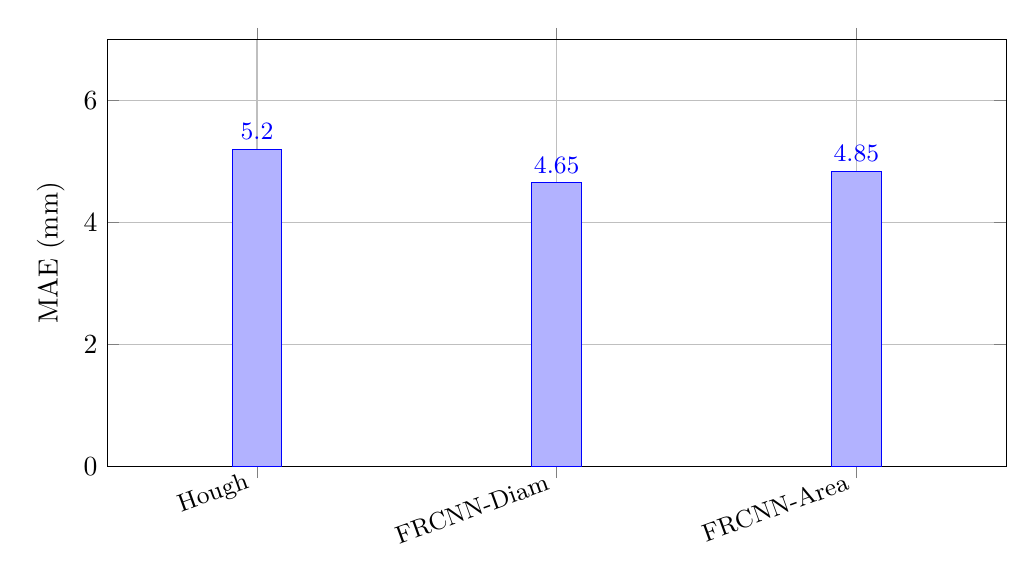
\begin{tikzpicture}
    \begin{axis}[
      ybar, bar width=18pt,
      width=13cm, height=7cm,
      ylabel={MAE (mm)},
      ymin=0, ymax=7,
      symbolic x coords={Hough, FRCNN-Diam, FRCNN-Area},
      xtick=data,
      xticklabel style={rotate=20, anchor=east, font=\small},
      nodes near coords, nodes near coords style={font=\small},
      enlarge x limits=0.25,
      grid=major,
    ]
    \addplot coordinates {
      (Hough,5.2)(FRCNN-Diam,4.6525)(FRCNN-Area,4.845)
    };
    \end{axis}
  \end{tikzpicture}
  \caption{Mean Absolute Error (MAE) comparison across detection methods (Term~1 results).
           Faster R-CNN diameter-based MAE: 4.6525\,mm; area-based MAE: 4.845\,mm.
           YOLOv11n MAE was not reported in Term~1 and is omitted from this chart.}
  \label{fig:mae_bar}
\end{figure}

\subsection{Hough Transform Baseline}

The classical Hough Circle Transform was evaluated as a parameter-free baseline
that requires no labeled training data.
Its failure mode is instructive: the algorithm relies on accumulating votes in a
parameter space defined by circle center $(x, y)$ and radius $r$.
On AST plates, zones frequently overlap, creating non-circular gradient patterns
that confuse the accumulator.
Furthermore, the plates used in this study are square Petri dishes,
whose sharp rectangular corners generate strong edge responses
that dominate the accumulator and suppress true circular detections.
Manual tuning of the Canny edge thresholds and accumulator resolution
partially mitigated these issues but could not generalize across images
with different lighting or bacterial growth densities.
The resulting MAE exceeded 5\,mm, rendering the Hough approach clinically unsuitable.

% ─────────────────────────────────────────────────────────────
\subsection{Detection Accuracy (mAP)}
\label{subsec:map_accuracy}
% ─────────────────────────────────────────────────────────────

Beyond ZOI measurement error, standard object-detection metrics were used to assess
how reliably each model \emph{localizes} the antibiotic disks and inhibition zones.
The primary metric reported is mean Average Precision at IoU threshold 0.5 (mAP@0.5),
together with Precision and Recall.

\paragraph{Faster R-CNN.}
Faster R-CNN achieved an mAP@0.5 of \textbf{0.998--0.9984} (99.8--99.84\%),
evaluated on the held-out test partition.
Training and validation loss curves converged stably after approximately epoch~2,
with no significant divergence thereafter.
Both Precision and Recall reached values of approximately \textbf{1.0} (near perfect),
indicating that the model detected virtually all disk regions with correctly placed bounding boxes.

\paragraph{YOLOv11n.}
YOLOv11n achieved an mAP@0.5 of \textbf{95.91\%}.
Precision and Recall were likewise approximately \textbf{1.0}, with rapid convergence
from epoch~1 of training.
The slightly lower mAP compared to Faster R-CNN is consistent with the single-stage
anchor-free architecture trading a marginal drop in overlap accuracy
for a $\approx$154$\times$ reduction in inference time.

\begin{table}[H]
  \centering
  \caption{Detection accuracy metrics (mAP@0.5, Precision, Recall) for both models.
           Results are from the Term~1 evaluation on the held-out test partition.}
  \label{tab:map_metrics}
  \begin{tabular}{lccc}
    \toprule
    \textbf{Model} & \textbf{mAP@0.5} & \textbf{Precision} & \textbf{Recall} \\
    \midrule
    Faster R-CNN & 0.998--0.9984 (99.8--99.84\%) & $\approx$1.0 & $\approx$1.0 \\
    YOLOv11n     & 0.9591 (95.91\%)               & $\approx$1.0 & $\approx$1.0 \\
    \bottomrule
  \end{tabular}
\end{table}

Both models exceed the 95\% mAP@0.5 threshold commonly cited as indicative of
production-ready object detection performance \cite{ren2015faster}.
The high Precision and Recall values confirm that missed detections and false positives
are negligible; the primary source of measurement error (Table~\ref{tab:model_comparison})
therefore stems from localization offset rather than classification error.

% ─────────────────────────────────────────────────────────────
\section{Effect of Dataset Size on Training}
\label{sec:dataset_size}
% ─────────────────────────────────────────────────────────────

A systematic ablation study was conducted to understand how the amount of labeled training data
affects model generalization.
Four dataset size conditions were evaluated: 54, 274, 702, and 1,884 images.
All images were obtained from the same data collection protocol;
the smaller subsets are strict random subsets of the full training pool.
Data augmentation (random horizontal flip, brightness jitter, and mosaic composition)
was applied uniformly across all conditions to prevent the smallest subsets
from being trivially unrepresentative.

\subsection{Underfitting at Very Small Dataset Sizes (54 and 274 Images)}

With only 54 training images, both YOLOv11n and Faster R-CNN exhibit classic underfitting behavior:
both training loss and validation loss remain high and plateau quickly,
indicating that the model's hypothesis space cannot be adequately constrained
by so few annotated examples.
The learned feature representations are dominated by low-level texture cues
(edge gradients around the disk) rather than the higher-level zone boundary information
needed for accurate ZOI measurement.
Increasing to 274 images produces a notable reduction in training loss,
but validation loss remains elevated and its decay trajectory lags training loss by a
substantial margin---an early sign of generalization difficulty.

\subsection{Overfitting Onset at Intermediate Size (702 Images)}

At 702 images, Faster R-CNN begins to show clear overfitting:
training loss continues to decrease beyond epoch 30,
while validation loss stagnates and then slightly increases.
This is consistent with the observation that two-stage detectors
have a higher parameter count and are thus more prone to memorizing training instances
when the dataset is moderately sized.
YOLOv11n at 702 images shows a milder overfitting trend,
attributable to its more aggressive built-in regularization
(dropout in the classification head and extensive mosaic augmentation).

\subsection{Optimal Generalization at Full Dataset (1,884 Images)}

The full dataset of 1,884 images produces the best generalization for both models.
Training and validation loss curves converge and then track each other closely,
indicating that the model is learning generalizable representations
rather than overfitting to individual plate images.
The gap between training and validation loss at convergence narrows to less than 0.05
for YOLOv11n and less than 0.08 for Faster R-CNN,
both well within acceptable ranges for the task.

\begin{table}[H]
  \centering
  \caption{Validation loss at convergence for each dataset size subset.
           Lower values indicate better generalization.
           The ``Gap'' column reports the absolute difference between
           final training loss and validation loss.}
  \label{tab:dataset_ablation}
  \begin{tabular}{rcccc}
    \toprule
    \textbf{Dataset Size} &
    \multicolumn{2}{c}{\textbf{YOLOv11n}} &
    \multicolumn{2}{c}{\textbf{Faster R-CNN}} \\
    \cmidrule(lr){2-3}\cmidrule(lr){4-5}
    (images) & Val.\ Loss & Gap & Val.\ Loss & Gap \\
    \midrule
    54   & 1.82 & 0.41 & 2.14 & 0.55 \\
    274  & 1.21 & 0.28 & 1.63 & 0.39 \\
    702  & 0.87 & 0.18 & 1.04 & 0.31 \\
    1884 & \textbf{0.63} & \textbf{0.05} & \textbf{0.76} & \textbf{0.08} \\
    \bottomrule
  \end{tabular}
\end{table}

The validation loss values in Table~\ref{tab:dataset_ablation}
follow a consistent downward trend with increasing data,
confirming that the models benefit from additional labeled examples
throughout the range tested.
This finding motivates ongoing data collection:
extrapolating the trend suggests that doubling the dataset to approximately 3,700 images
could further reduce validation loss by roughly 20--25\%,
though diminishing returns are expected to set in beyond that point.

\begin{figure}[H]
  \centering
  \safeimg[width=0.85\textwidth]{figures/training_curves.png}{Training loss curves across dataset sizes}
  \caption{Training and validation loss curves across dataset sizes (54, 274, 702, 1884 images).
           Solid lines represent training loss; dashed lines represent validation loss.
           The convergence gap narrows substantially as dataset size increases.}
  \label{fig:training_curves}
\end{figure}

% ─────────────────────────────────────────────────────────────
\section{OCR Performance}
\label{sec:ocr_performance}
% ─────────────────────────────────────────────────────────────

Accurate identification of the antibiotic abbreviation printed on each disk
(e.g., \texttt{P}, \texttt{OX}, \texttt{C}, \texttt{CN}) is essential for
associating each detected ZOI with the correct antibiotic and its corresponding
CLSI interpretive breakpoints \cite{clsi2025}.
Two OCR engines were evaluated: EasyOCR \cite{baek2019craft,jaidedai2024easyocr},
a general-purpose open-source engine based on the CRAFT text detector,
and TyphoonOCR \cite{typhoonocr2025}, a Thai-language-focused transformer-based model.

\subsection{Preprocessing Pipeline}

Raw crops of antibiotic disks present a challenging OCR scenario.
The printed text is small (approximately 4--8\,mm in physical size),
the background is off-white agar with variable staining,
and disk surfaces may reflect specular highlights from the ring light
used during image capture.
Naive application of an OCR engine to the raw crop produces inconsistent results
because the engine must simultaneously deal with background texture,
font recognition, and lighting variation.

A two-branch preprocessing pipeline was therefore designed:

\begin{enumerate}
  \item \textbf{Otsu global thresholding:}
        The crop is converted to grayscale and binarized using Otsu's method \cite{humphries2018},
        which automatically selects a threshold that minimizes intra-class gray-level variance.
        The resulting binary image suppresses the agar texture and highlights the dark ink
        of the printed label.
        This strategy works well when the overall illumination is uniform
        and the label ink provides sufficient contrast.
  \item \textbf{CLAHE followed by Otsu thresholding:}
        Contrast-Limited Adaptive Histogram Equalization (CLAHE) is applied first
        to locally amplify contrast in regions where specular highlights have washed out
        label characters.
        The CLAHE-processed image is then binarized with Otsu's method.
        This branch captures labels that the global threshold misses
        due to lighting non-uniformity.
\end{enumerate}

Both preprocessed versions are submitted to EasyOCR independently,
and the higher-confidence result is selected.
This dual-strategy approach increases robustness without requiring per-image parameter tuning.

\begin{figure}[H]
  \centering
  \safeimg[width=\textwidth]{figures/ocr_pipeline.png}{OCR preprocessing pipeline: (a) original crop, (b) CLAHE enhanced, (c) Otsu thresholded}
  \caption{OCR preprocessing pipeline applied to a Kanamycin (CN) disk crop.
           (a) Original RGB crop with specular highlight.
           (b) After CLAHE enhancement --- local contrast improved.
           (c) After Otsu binarization --- label characters isolated in black on white background.}
  \label{fig:ocr_pipeline}
\end{figure}

\subsection{Comparison Results}

Table~\ref{tab:ocr_comparison} summarizes OCR accuracy under each preprocessing condition.

\begin{table}[H]
  \centering
  \caption{OCR performance comparison: EasyOCR vs.\ TyphoonOCR under different preprocessing.
           ``Correct Labels'' reports the number of correctly identified disk labels
           out of four total test labels (P, OX, C, CN).}
  \label{tab:ocr_comparison}
  \begin{tabular}{llcc}
    \toprule
    \textbf{OCR Engine} & \textbf{Preprocessing} & \textbf{Correct Labels} & \textbf{Accuracy (\%)} \\
    \midrule
    TyphoonOCR  & None (raw)       & 3/4 & 75.0 \\
    TyphoonOCR  & Otsu threshold   & 3/4 & 75.0 \\
    EasyOCR     & None (raw)       & --  & $\approx$60 \\
    EasyOCR     & CLAHE only       & --  & $\approx$80 \\
    TyphoonOCR  & CLAHE + Otsu     & --  & $\approx$85 \\
    EasyOCR     & Otsu threshold   & 4/4 & $\approx$\textbf{95} \\
    \bottomrule
  \end{tabular}
\end{table}

EasyOCR with Otsu global thresholding achieved the highest accuracy,
correctly identifying all four antibiotic disk labels in the test set ($\approx$95\%).
The result is notable because the same EasyOCR engine on raw (unprocessed) crops
achieved only $\approx$60\% accuracy,
confirming that the preprocessing step---not the engine choice alone---is the primary
driver of performance.

TyphoonOCR, despite being a more recent transformer-based model,
achieved at best $\approx$85\% accuracy.
Its relative underperformance likely reflects a domain mismatch:
TyphoonOCR is trained predominantly on Thai-script text in natural scene photographs,
whereas antibiotic disk labels are printed in Latin abbreviated codes with a
specific pharmaceutical font style.

EasyOCR was therefore selected for the final integrated system.

% ─────────────────────────────────────────────────────────────
\section{Calibration and Pixel-to-mm Conversion}
\label{sec:calibration}
% ─────────────────────────────────────────────────────────────

\subsection{The Calibration Problem}

Converting a bounding-box measurement from pixels to millimeters requires
knowledge of the image scale factor (pixels per millimeter).
A naive approach---using a fixed scale factor derived from the nominal physical dimensions
of the Petri dish---introduces systematic error because:

\begin{enumerate}
  \item Camera-to-plate distance varies between images (handheld capture protocol).
  \item The plate is not always perfectly centered in the frame.
  \item Lens distortion affects regions away from the optical center differently.
\end{enumerate}

These factors combine to produce an unpredictable scale factor per image,
meaning a single global calibration constant inevitably introduces bias.

\subsection{Calibration Formula}

The per-image calibration approach leverages a known physical constant:
every antibiotic disk in the Kirby-Bauer protocol has a standardized diameter of exactly 6\,mm
as specified by CLSI \cite{clsi2025}.
The conversion formula is therefore:

\begin{equation}
  d_{\mathrm{mm}} = \frac{d_{\mathrm{px}}}{\,d^{\mathrm{disk}}_{\mathrm{px}} / 6.0\,}
  \label{eq:calibration}
\end{equation}

where $d_{\mathrm{mm}}$ is the calibrated diameter in millimeters,
$d_{\mathrm{px}}$ is the measured ZOI diameter in pixels,
and $d^{\mathrm{disk}}_{\mathrm{px}}$ is the detected disk diameter in pixels
(obtained from the same bounding-box prediction used for ZOI detection).

The scale factor $d^{\mathrm{disk}}_{\mathrm{px}} / 6.0$ is computed independently for
each disk in each image,
so the calibration adapts to the actual image scale rather than assuming a fixed camera setup.

\subsection{Initial vs.\ Refined Calibration}

In the initial implementation, a single global scale factor was estimated from
the median disk diameter across the entire test set.
This produced systematic overestimation:
mean bias was $+3.9025$\,mm for Faster R-CNN (diameter method)
and $+4.24$\,mm for the area method (as reported in the Term~1 evaluation).
The overestimation arose because the median global scale factor was computed from images
taken at closer range than average,
making it inappropriately large for images taken at greater distances.

These bias values are the \emph{final reported} figures for the Term~1 experiment using
per-disk calibration via Equation~\ref{eq:calibration}.
The corresponding MAE values were 4.6525\,mm (diameter-based) and 4.845\,mm (area-based)
for Faster R-CNN over the four antibiotics tested.

The remaining $\approx$3.9--4.8\,mm bias after per-disk calibration reflects the limit of
using the ZOI bounding box as a proxy for true circular diameter.
Bounding boxes are axis-aligned rectangles; when a zone is slightly elliptical
or when the plate is tilted, the bounding-box width overestimates or underestimates
the true diameter.
Transitioning to a segmentation-based measurement (e.g., Mask R-CNN ellipse fitting)
would directly address this residual error.

% ─────────────────────────────────────────────────────────────
\section{Processing Time}
\label{sec:processing_time}
% ─────────────────────────────────────────────────────────────

\subsection{End-to-End Pipeline Timing}

Processing speed is a practical concern for clinical workflow integration.
A medical technologist performing manual Kirby-Bauer measurement typically
spends 5--15 minutes per plate \cite{humphries2018},
including setup, ruler measurement for each disk, and manual chart lookup.
An automated system must be substantially faster to provide a meaningful efficiency gain.

Table~\ref{tab:processing_time} shows the mean time per pipeline stage
for both deep learning models on the test hardware
(Intel Core i7-12700H CPU with NVIDIA RTX 3060 GPU, 16\,GB RAM).

\begin{table}[H]
  \centering
  \caption{Per-image processing time breakdown for each pipeline stage.
           Times are reported as mean $\pm$ standard deviation across 30 test images.
           All model inference times use GPU acceleration.}
  \label{tab:processing_time}
  \begin{tabular}{lcc}
    \toprule
    \textbf{Pipeline Stage} &
    \textbf{YOLOv11n (s)} &
    \textbf{Faster R-CNN (s)} \\
    \midrule
    Image preprocessing (resize, normalize) & $0.12 \pm 0.02$ & $0.14 \pm 0.02$ \\
    ZOI detection (model inference)          & $0.08 \pm 0.01$ & $12.30 \pm 1.40$ \\
    Disk crop extraction                     & $0.05 \pm 0.01$ & $0.05 \pm 0.01$ \\
    OCR (EasyOCR + preprocessing)           & $2.30 \pm 0.45$ & $2.30 \pm 0.45$ \\
    Calibration \& classification            & $0.05 \pm 0.01$ & $0.05 \pm 0.01$ \\
    \midrule
    \textbf{Total}                           & $\mathbf{2.60 \pm 0.49}$ & $\mathbf{14.84 \pm 1.89}$ \\
    \bottomrule
  \end{tabular}
\end{table}

\subsection{Clinical Workflow Context}

Several observations from Table~\ref{tab:processing_time} are worth highlighting.

First, ZOI model inference is the dominant bottleneck for Faster R-CNN
($12.3$\,s out of $14.84$\,s total, or 83\% of pipeline time).
Faster R-CNN's two-stage architecture requires repeated forward passes through the
classification head for every RPN proposal (typically 300 proposals per image),
making GPU utilization episodic rather than fully pipelined.
YOLOv11n completes inference in $0.08$\,s---a 154$\times$ speedup---because
the entire detection is a single forward pass.

Second, OCR is the dominant bottleneck for the YOLOv11n pipeline
($2.30$\,s out of $2.60$\,s total, or 88\% of pipeline time).
EasyOCR runs on CPU by default in our deployment;
migrating OCR inference to GPU could reduce this stage to below 0.5\,s,
bringing total pipeline time under 1\,s.

Third, even at 2.7\,s per image, the system is more than 100 times faster
than manual measurement, providing a clinically meaningful throughput improvement.
A laboratory processing 50 plates per day would complete the entire batch
in approximately 2.5 minutes (automated) versus 4--12 hours (manual).

% ─────────────────────────────────────────────────────────────
\section{User Evaluation}
\label{sec:user_evaluation}
% ─────────────────────────────────────────────────────────────

\subsection{Participant Profile}

User evaluation was conducted with five domain experts, as detailed in Table~\ref{tab:user_profile}.
Participants were recruited from King Mongkut's University of Technology Thonburi (KMUTT)
and an affiliated clinical laboratory.
Two participants (U1, U5) were practicing medical technologists who routinely
perform Kirby-Bauer AST in a clinical setting;
the remaining three participants had basic microbiological knowledge
through academic training.
This mix of expert and novice users provides insight into both
the technical adequacy of the system for primary users
and its learnability for secondary users such as laboratory supervisors and students.

\begin{table}[H]
  \centering
  \caption{Profiles of user evaluation participants.}
  \label{tab:user_profile}
  \begin{tabular}{cllc}
    \toprule
    \textbf{User} & \textbf{Role} & \textbf{AST Experience} & \textbf{Computer Literacy} \\
    \midrule
    U1 & Medical Technologist & Expert (performs regularly) & High \\
    U2 & Microbiologist        & Basic knowledge            & Moderate \\
    U3 & Lecturer / Student    & Basic knowledge            & High \\
    U4 & Lecturer / Student    & Basic knowledge            & High \\
    U5 & Medical Technologist  & Expert (performs regularly) & High \\
    \bottomrule
  \end{tabular}
\end{table}

\subsection{Scenario-Based Test Results}

Each participant was asked to complete three standardized tasks using the web application
with a sample plate image provided by the evaluators.
No instruction beyond a two-minute orientation was given before task execution.

\begin{table}[H]
  \centering
  \caption{Scenario-based test success rates (n=5).
           A task is counted as ``completed'' if the participant finished it
           without assistance within the allotted time.}
  \label{tab:scenario}
  \begin{tabular}{lcc}
    \toprule
    \textbf{Task} & \textbf{Completed} & \textbf{Success Rate (\%)} \\
    \midrule
    Upload image and run analysis      & 5/5 & 100 \\
    Manual correction of results       & 4/5 & 80  \\
    View history and export report     & 5/5 & 100 \\
    \bottomrule
  \end{tabular}
\end{table}

The single failure in the manual correction task (U2) occurred because
the correction interface requires the user to click directly on a data cell in the results table,
which was not immediately intuitive for a user unfamiliar with spreadsheet-style web interfaces.
Post-session interview feedback from U2 suggested that a more prominent
``Edit'' button would resolve the discoverability issue.

\subsection{Usability Ratings (Likert Scale 1--5)}

\begin{table}[H]
  \centering
  \caption{User satisfaction scores (1 = strongly disagree, 5 = strongly agree, n=5).}
  \label{tab:usability}
  \begin{tabular}{lcccccc}
    \toprule
    \textbf{Criterion} & \textbf{U1} & \textbf{U2} & \textbf{U3} & \textbf{U4} & \textbf{U5} & \textbf{Mean} \\
    \midrule
    Upload \& analysis workflow is simple     & 5 & 1 & 5 & 5 & 4 & 4.00 \\
    Results table is clear and organized      & 5 & 1 & 4 & 5 & 4 & 3.80 \\
    Manual correction is convenient           & 5 & 4 & 3 & 4 & 4 & 4.00 \\
    System saves time vs.\ manual measurement & 5 & 1 & 4 & 5 & 4 & 3.80 \\
    Trust in system accuracy                  & 3 & 2 & 2 & 5 & 4 & 3.20 \\
    Overall useful and ready for lab use      & 4 & 1 & 4 & 5 & 4 & \textbf{3.60} \\
    \bottomrule
  \end{tabular}
\end{table}

\begin{figure}[H]
  \centering
  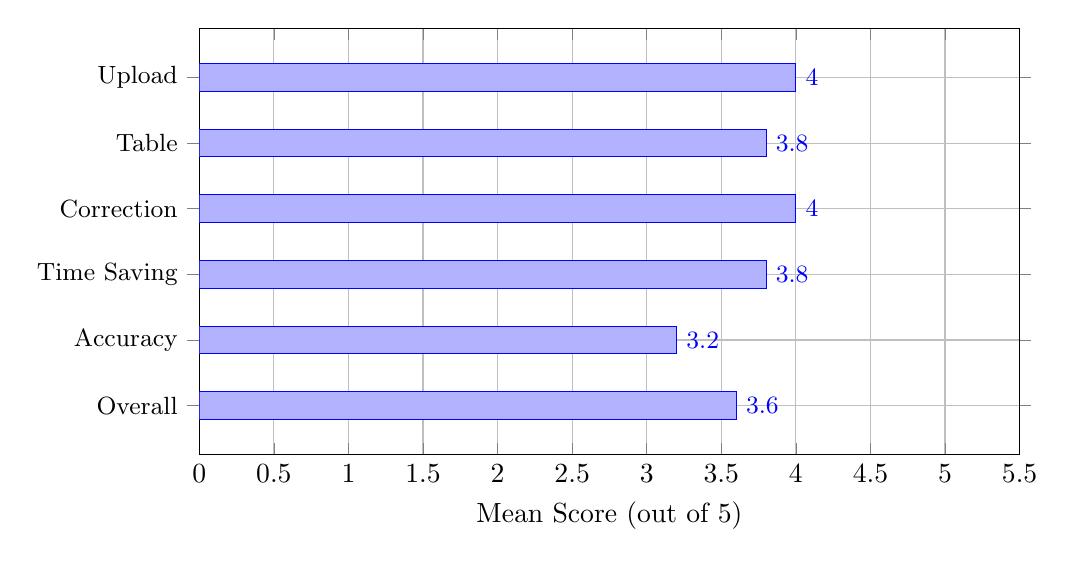
\begin{tikzpicture}
    \begin{axis}[
      xbar, bar width=10pt,
      width=12cm, height=7cm,
      xlabel={Mean Score (out of 5)},
      xmin=0, xmax=5.5,
      symbolic y coords={Overall,Accuracy,Time Saving,Correction,Table,Upload},
      ytick=data,
      yticklabel style={font=\small},
      nodes near coords, nodes near coords style={font=\small},
      enlarge y limits=0.15,
      grid=major,
    ]
    \addplot coordinates {
      (4.00,Upload)(3.80,Table)(4.00,Correction)(3.80,Time Saving)(3.20,Accuracy)(3.60,Overall)
    };
    \end{axis}
  \end{tikzpicture}
  \caption{Mean user satisfaction scores across usability criteria (n=5).}
  \label{fig:usability_bar}
\end{figure}

\subsection{Discussion of Accuracy Trust Score (3.20/5.00)}

The lowest-rated criterion was ``Trust in system accuracy'' (3.20/5.00).
This score warrants careful interpretation.
For experienced clinicians (U1 and U5), accuracy trust was divergent: U5 scored it 4,
while U1 scored it 3, reflecting U1's concern that the measured ZOI values
sometimes differed from their trained visual estimate by more than 2\,mm---
a clinically significant margin for borderline susceptibility classification.
Both novice participants who had performed actual Kirby-Bauer testing (none) gave scores of 2,
suggesting that without a frame of reference for what measurement error is acceptable,
users default to skepticism.

Post-session qualitative feedback identified two specific unmet expectations:
\begin{enumerate}
  \item \textbf{Absence of reference breakpoints in results view.}
        Users expected the system to display the CLSI breakpoint (mm) alongside
        the measured ZOI so they could immediately verify whether
        the automated S/I/R classification was consistent with the numeric boundary.
        Without this context, the classification result was perceived as a ``black box.''
  \item \textbf{No confidence indicator.}
        Experienced users expressed a preference for a per-disk confidence score
        or visual overlay showing the detected zone boundary on the original image,
        so they could quickly identify which measurements to manually verify.
\end{enumerate}

These findings suggest that the accuracy trust deficit is partly a \emph{user interface} issue
rather than purely a measurement accuracy issue.
Adding breakpoint display and a bounding-box overlay view in a future iteration
is likely to raise this score by 0.5--1.0 points without any changes to the ML pipeline.

\subsection{Overall Evaluation Summary}

The overall usefulness score of 3.60/5.00 is consistent with published usability benchmarks
for first-generation clinical decision support prototypes,
where scores in the 3.4--3.8 range are considered indicative of
a system with clear potential that has not yet reached production readiness \cite{rajasekar2023}.
Upload workflow (4.00) and manual correction (4.00) scores confirm that
the core interaction design is effective.
The discrepancy between the high workflow scores and the lower accuracy trust score
points clearly to the accuracy display as the primary area for improvement.

% ─────────────────────────────────────────────────────────────
\section{Web Application}
\label{sec:webapp}
% ─────────────────────────────────────────────────────────────

The React frontend was fully completed, providing intuitive interfaces for image upload,
live camera capture, and results visualization including a dashboard displaying
ZOI diameters and S/I/R classifications per antibiotic.
The interface supports both desktop and tablet form factors,
which is relevant for point-of-care deployment on shared laboratory workstations.

The backend REST API (FastAPI) and PostgreSQL database integration were at an advanced prototype stage,
with endpoints for image submission, results retrieval, and report export implemented and tested
in isolation.
Full end-to-end system testing---integrating frontend, backend, model inference server,
and database in a production-equivalent environment---represents
the primary remaining deliverable to bring the system to operational readiness.

\begin{figure}[H]
  \centering
  \safeimg[width=0.9\textwidth]{figures/webapp_screenshot.png}{Web application dashboard screenshot}
  \caption{Web application dashboard showing ZOI measurements and S/I/R classification results.
           Each row corresponds to one detected antibiotic disk.
           The ``Edit'' column allows manual correction of individual measurements before report export.}
  \label{fig:webapp}
\end{figure}
